\section{Introduction}\label{introduction}

\begin{itemize}
\itemsep1pt\parskip0pt\parsep0pt
\item
  Topic
\item
  Motivation
\item
  Aims
\end{itemize}

\section{Data Sources}\label{data-sources}

\begin{itemize}
\itemsep1pt\parskip0pt\parsep0pt
\item
  kurze Beschreibung der drei Datenquellen
\item
  vielleicht die (konzeptuelle) Beschreibung der Download Prozesse auch
  hier?
\end{itemize}

\section{Data Model}\label{data-model}

\begin{figure}[htbp]
\centering
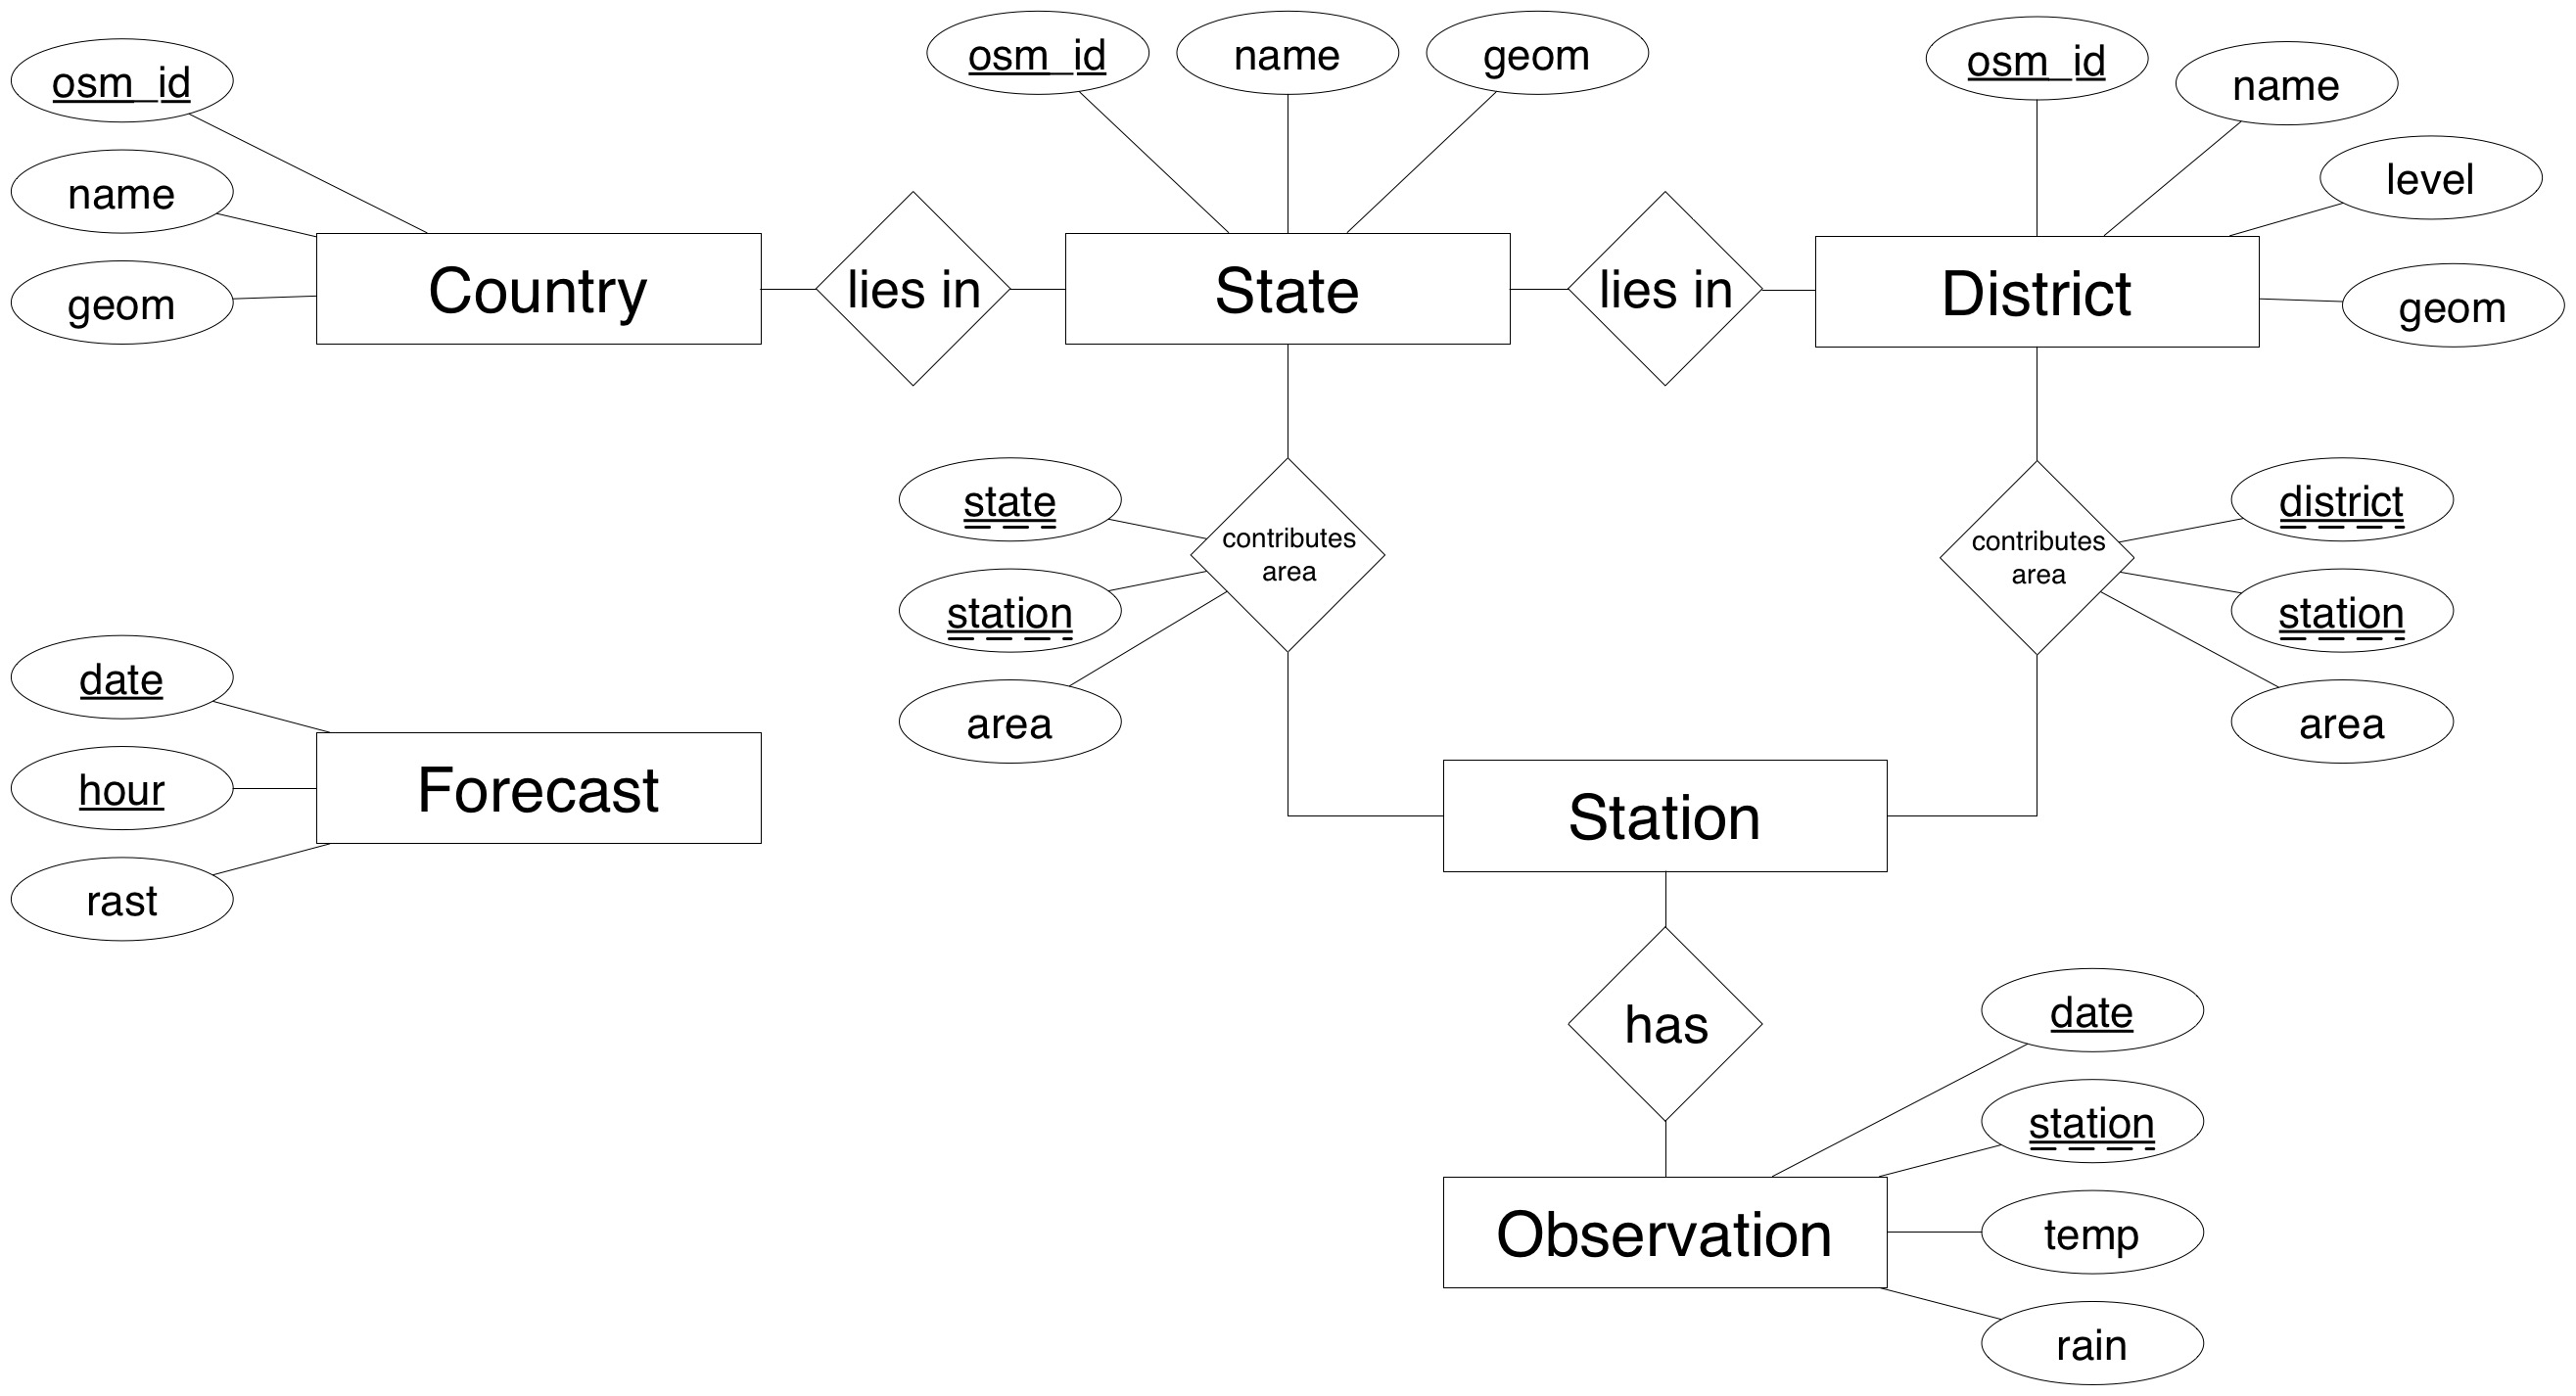
\includegraphics{pictures/er-model.jpg}
\caption{ER Model}
\end{figure}

\begin{itemize}
\itemsep1pt\parskip0pt\parsep0pt
\item
  ER Modell plus 2-3 Sätze
\end{itemize}

\section{Architecture}\label{architecture}

\begin{itemize}
\itemsep1pt\parskip0pt\parsep0pt
\item
  Bild + Beschreibung
\end{itemize}

\section{Optimizations}\label{optimizations}

\begin{itemize}
\itemsep1pt\parskip0pt\parsep0pt
\item
  Indices
\item
  Contrib Tables
\item
  Topology Simplification
\end{itemize}

\section{Usage}\label{usage}

As mentioned in the Architecure section, the weather map is displayed
with HTML5 and controlled with JavaScript. It has been developed as a
control for the Leaflet library and tested on Google Chrome and
Chromium. Other browsers are not offically supported.

By default Leaflet is using a zoom and a layer selection control.
Instead of rendering the basetiles ourselves, we are using the freely
available
\href{http://wiki.openstreetmap.org/wiki/Tile_usage_policy}{OSM Tile
Server} and tiles generated for free by
\href{https://www.mapbox.com/}{Mapbox}. The desired basetile layer can
be selected as seen in fig. ??

\begin{figure}[htbp]
\centering
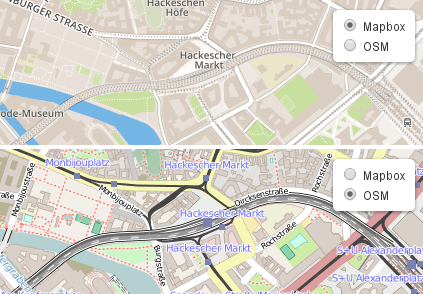
\includegraphics{pictures/screenshot-baselayer.png}
\caption{Layer Selection}
\end{figure}

The map can also be panned and zoommed by using a pointing device
(e.g.~mouse).

The displayed weather data can be set by an additional control as seen
in fig. ??

\begin{figure}[htbp]
\centering
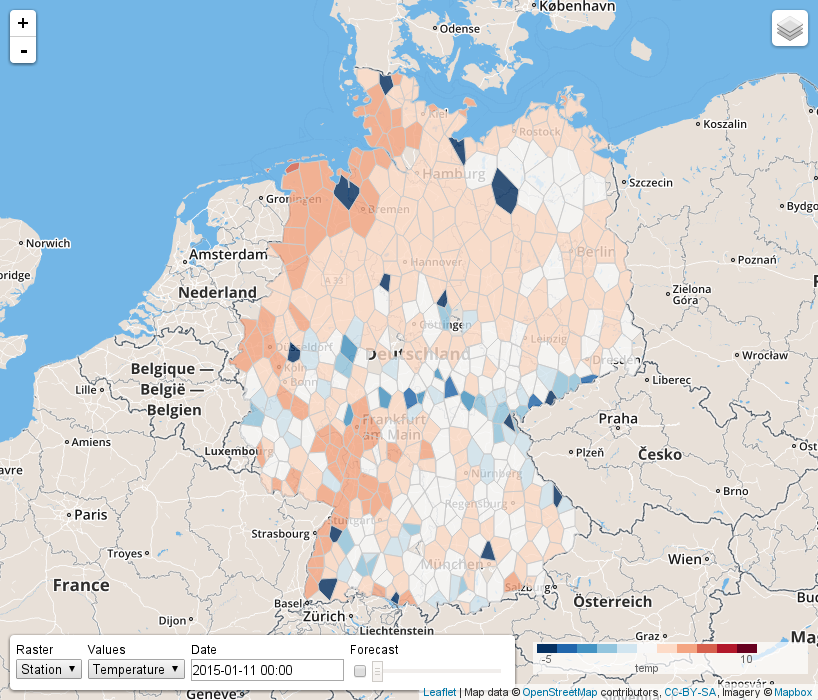
\includegraphics{pictures/screenshot-control.png}
\caption{Weather Control}
\end{figure}

It allows to choose either temperatures or reciproc.?? rainfall for a
certain day. The day can be selected with an interactive datetime picker
as seen in fig. ??

\begin{figure}[htbp]
\centering
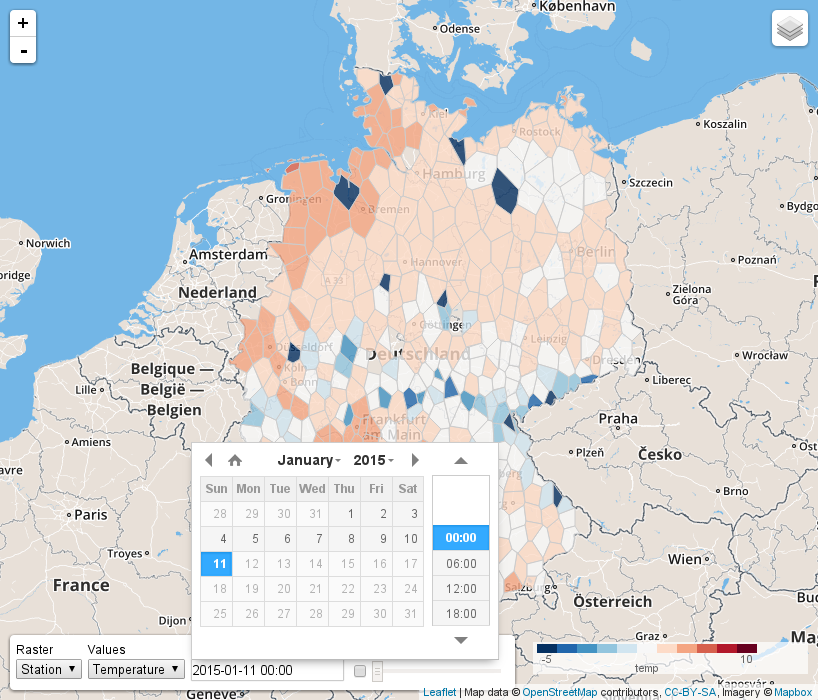
\includegraphics{pictures/screenshot-control-datetime.png}
\caption{Datetime Picker}
\end{figure}

The selected date and time is also used to pick the computed GFS used to
display forecasts. If the forecast box is checked, the forecasts slider
is activated and allows to select point of forecast in hours, starting
from the chosen date and time.

As mentioned before, the data can be displayed for different rasters: a
voronoi tesselation based on offical weather stations, german states or
districts. The desired raster can be selected with the control. Once the
selection did change, the weather control is loading the matching data
from the backend via a JSON interface and displays the raster on the
map.

\begin{figure}[htbp]
\centering
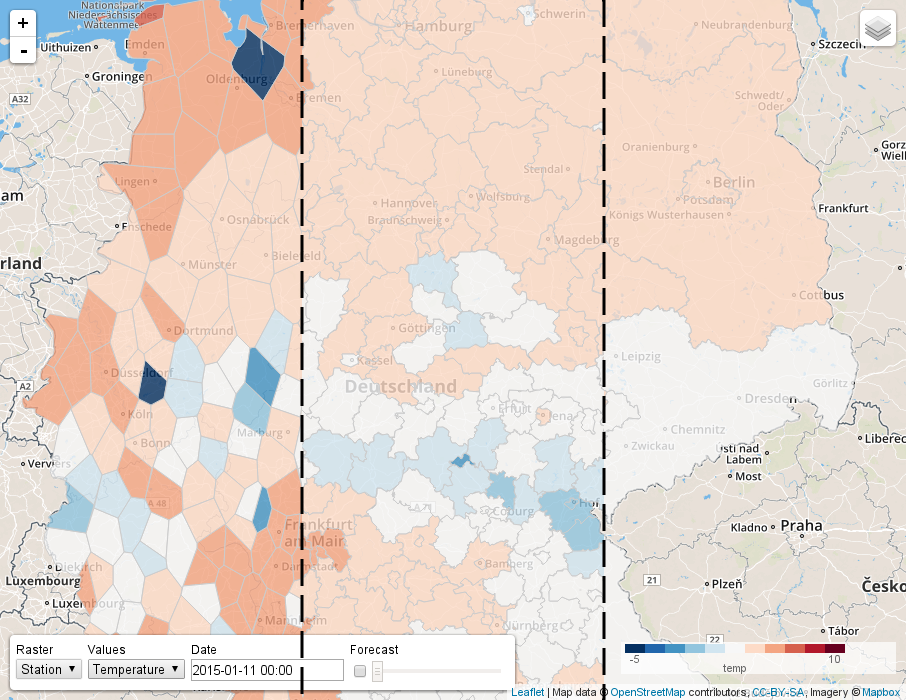
\includegraphics{pictures/screenshot-raster.png}
\caption{Raster comparison}
\end{figure}

The cells are colored according to selected data and a legend is shown
on the lower right for reference (see fig. ?? - ??)

\begin{figure}[htbp]
\centering
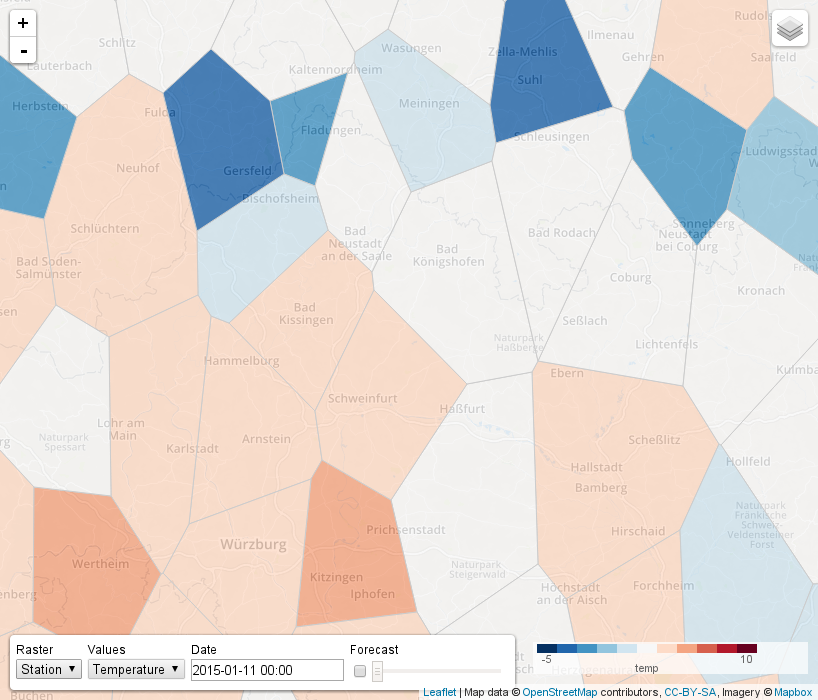
\includegraphics{pictures/screenshot-legend-temp.png}
\caption{Temperature Legend}
\end{figure}

\begin{figure}[htbp]
\centering
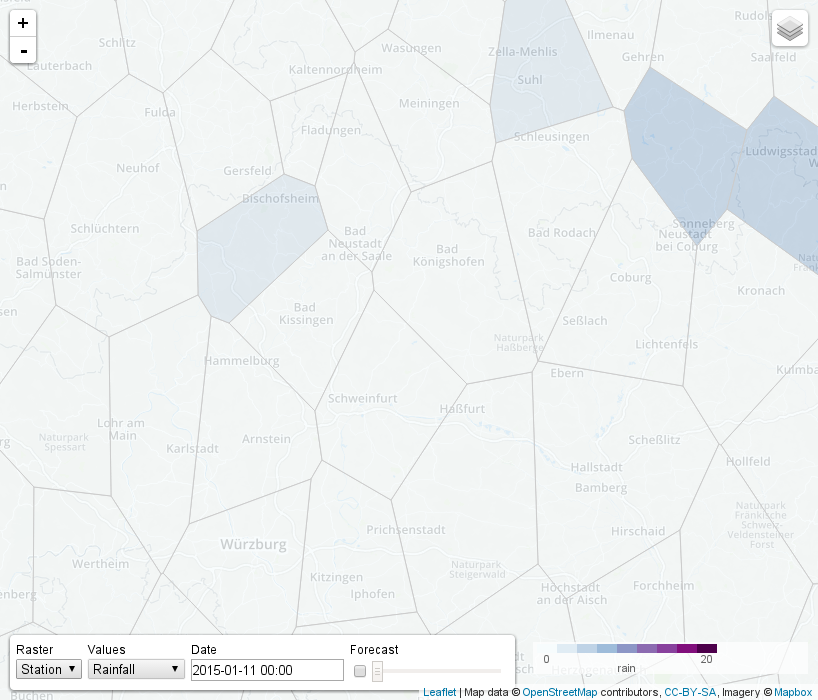
\includegraphics{pictures/screenshot-legend-rain.png}
\caption{Rainfall Legend}
\end{figure}

Each cell is clickable and highlights it's border or, in case of the
voronoi tesselation, the position of the weather station. Furthermore a
popup is shown, which is showing additional data associated to the
selected cell by calling the backends JSON interface.

\begin{figure}[htbp]
\centering
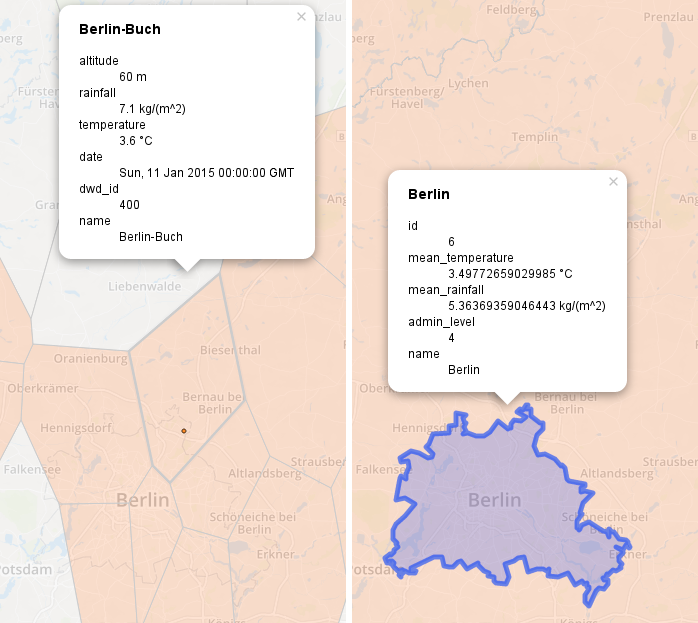
\includegraphics{pictures/screenshot-popup.png}
\caption{Popup}
\end{figure}

Currently this is just the alphanumerical attributes, but could be used
to show automatically generated temperature timelines or recent webcam
photos or \ldots{} {[}\textbf{TODO: noch mehr ausblick kram\ldots{}}{]}

\begin{itemize}
\itemsep1pt\parskip0pt\parsep0pt
\item
  kurze Beschreibung was wir Anzeigen können
\item
  Screenshots (da sind sie glaub ich geil drauf)
\end{itemize}

\section{Conclusion}\label{conclusion}

\begin{itemize}
\itemsep1pt\parskip0pt\parsep0pt
\item
  lessons learned
\end{itemize}

\section{Appendix}\label{appendix}

\begin{itemize}
\itemsep1pt\parskip0pt\parsep0pt
\item
  Literature (if any)
\item
  Setup Guide
\item
  Link to Repo
\end{itemize}
